\section{Experimentos}
\subsection{Secuencias de desarme utilizadas}

\begin{table}
	\centering
	\begin{tabular}{|r|c|}
		\hline
		ID & Desarme \\ \hline \hline
		 1 & R2 D1 L3 D3 R1 B3 D2 F2 L1 R2 U3 R2 F2 D2 F1 U3 F2 D3 U3 L1 B2 L2 R2 U3 R1 U2 F2 D3 R2 U3 \\ \hline
		 2 & D1 F2 D3 B2 L1 B2 F2 D3 B2 L3 F2 U1 R2 B2 U3 B3 D1 R2 F3 D3 L2 R2 F2 L3 D2 U1 R2 F3 L3 B1 \\ \hline
		 3 & L2 U2 F1 R2 F3 R2 F3 L1 B2 R2 B1 F2 D2 U2 L2 R2 D2 B2 U3 F1 U3 L3 R2 D1 U1 B1 F3 L2 R3 F2 \\ \hline
		 4 & B2 F3 R1 D2 U1 L3 R2 B1 U1 F2 U2 B3 L3 B1 F1 D3 U2 R3 B3 R3 F1 R2 D1 L3 F1 L2 R3 B1 F1 U1 \\ \hline
		 5 & D1 R1 U2 L3 B2 R3 B3 R2 B3 L1 U1 B3 F2 L1 R1 U3 B1 U1 R2 D1 U1 B2 D2 U3 B2 U3 L2 R3 D3 F2 \\ \hline
		 6 & U2 L3 U3 L3 R2 U3 B2 R2 B1 U1 L3 R3 D1 R3 D2 F2 R2 B1 F3 L1 B2 D1 U1 L3 U1 R2 F3 D2 F1 R1 \\ \hline
		 7 & B1 F2 R3 F1 L1 B3 F2 D2 L3 R2 F3 L3 R1 D2 U1 F1 R2 F2 U3 R1 F1 D2 B2 R1 B1 R1 D3 U1 F3 R1 \\ \hline
		 8 & D1 U1 L1 U2 L1 R1 B1 F1 R1 D3 U3 L3 R3 D1 U2 B3 R1 U1 R1 D1 B3 F1 U2 B2 F2 D1 U1 L2 D3 F2 \\ \hline
		 9 & U3 R1 D3 B2 F2 U2 B3 L2 R2 F3 D2 U3 F3 L2 R1 D2 B3 D2 L2 U2 L1 U1 B1 F1 D2 L3 B2 U2 L3 U1 \\ \hline
		10 & L3 R1 B3 F3 U3 F2 L3 R1 D3 F3 U3 F1 D3 U3 B2 R3 B3 F3 R3 B2 F1 D2 B3 D1 B1 R1 F1 R2 U1 L2 \\ \hline
		11 & L3 B2 R1 B3 D1 F2 L3 B1 R1 B2 D3 B1 U1 F3 R2 D3 L2 R2 U1 B2 U2 R1 D3 U3 F1 R2 B3 F1 U2 F3 \\ \hline
		12 & D3 U1 L1 R1 B1 F1 R1 F2 U2 F3 L3 R2 D2 U2 F3 U3 F3 L3 B3 F1 U3 L3 B2 F1 L3 D1 L3 R2 D2 R3 \\ \hline
		13 & R3 D2 L1 R1 F1 L2 B1 F2 L2 D1 L2 R2 B1 F2 U2 B3 L1 U3 F1 D3 F2 L1 D1 F1 D1 F3 R1 U1 L3 F3 \\ \hline
		14 & B3 L2 R2 B2 F2 L1 F3 U1 F3 L3 U3 B2 F3 U2 F3 L1 D2 L3 R2 D2 F3 L2 D2 F1 D2 B3 R2 F2 D2 U1 \\ \hline
		15 & F1 U2 R3 U3 B1 F2 R2 D1 U1 L3 R3 B3 F1 D3 B3 F1 L3 B1 R1 U2 F3 U1 R3 D1 F3 D3 U2 L2 D2 B1 \\ \hline
		16 & F2 D2 L3 D3 L1 R1 D3 F3 D2 B3 U2 L1 D3 U1 L1 D3 B1 U1 R1 D3 R3 U1 R2 D3 L1 B1 R1 F3 L2 D1 \\ \hline
		17 & B3 F2 U1 F2 L1 R1 D1 U3 F1 U2 F2 L1 R1 D2 B1 D1 F2 R2 U3 R1 D2 U2 F3 L1 R3 F3 L3 R2 F2 L2 \\ \hline
		18 & B1 F3 D3 L3 B1 F2 R1 D3 L2 R1 F1 D2 F1 R3 F2 U3 B1 F2 D1 L3 U3 B2 F2 D3 L2 D3 U3 B1 U2 L1 \\ \hline
		19 & L3 U1 F1 D3 U3 R3 B2 U1 R2 F2 R3 B1 R1 U1 L2 B3 F3 U1 L2 R1 U3 B2 L3 U1 F1 R3 B1 L1 F2 L1 \\ \hline
		20 & D3 L3 R3 U2 R1 F2 L2 D3 F1 D3 R1 D2 U2 R2 F2 L2 R2 F3 R2 D3 B1 U1 B2 L1 R3 F3 D2 F1 R1 F2 \\ \hline
	\end{tabular}
	\caption{Desarmes utilizados para la experimentos de visión.}
	\label{vision}
\end{table}

\begin{table}
	\centering
	\begin{tabular}{|r|c|}
		\hline
		ID & Desarme \\ \hline \hline
		1 & R2 \\ \hline
		2 & D1 F2 \\ \hline
		3 & L2 U2 F1 \\ \hline
		4 & B2 F3 R1 D2 \\ \hline
		5 & D1 R1 U2 L3 B2 \\ \hline
		6 & U2 L3 U3 L3 R2 U3 \\ \hline
		7 & B1 F2 R3 F1 L1 B3 F2 \\ \hline
		8 & D1 U1 L1 U2 L1 R1 B1 F1 \\ \hline
		9 & U3 R1 D3 B2 F2 U2 B3 L2 R2 \\ \hline
	   10 & L3 R1 B3 F3 U3 F2 L3 R1 D3 F3 \\ \hline
	   11 & L3 B2 R1 B3 D1 F2 L3 B1 R1 B2 D3 \\ \hline
	   12 & D3 U1 L1 R1 B1 F1 R1 F2 U2 F3 L3 R2 \\ \hline
	   13 & R3 D2 L1 R1 F1 L2 B1 F2 L2 D1 L2 R2 B1 \\ \hline
	   14 & B3 L2 R2 B2 F2 L1 F3 U1 F3 L3 U3 B2 F3 U2 \\ \hline
	   15 & F1 U2 R3 U3 B1 F2 R2 D1 U1 L3 R3 B3 F1 D3 B3 \\ \hline
	   16 & F2 D2 L3 D3 L1 R1 D3 F3 D2 B3 U2 L1 D3 U1 L1 D3 \\ \hline
	   17 & B3 F2 U1 F2 L1 R1 D1 U3 F1 U2 F2 L1 R1 D2 B1 D1 F2 \\ \hline
	   18 & B1 F3 D3 L3 B1 F2 R1 D3 L2 R1 F1 D2 F1 R3 F2 U3 B1 F2 \\ \hline
	   19 & L3 U1 F1 D3 U3 R3 B2 U1 R2 F2 R3 B1 R1 U1 L2 B3 F3 U1 L2 \\ \hline
	   20 & D3 L3 R3 U2 R1 F2 L2 D3 F1 D3 R1 D2 U2 R2 F2 L2 R2 F3 R2 D3 \\ \hline
	\end{tabular}
	\caption{Desarmes utilizados para la experimentos de manipulación.}
	\label{manipulation}
\end{table}

\subsection{Detalle experimentos visión}
La tabla\ref{visionerrors} indica los facelet específicos donde el algoritmo de visión desarrollado se equivocó.
Un subíndice, cuando existe, indica el valor correcto, cuando no quiere decir que el facelet fue correctamente identificado.
\begin{table}
	\centering
		\begin{tabular}{|r|r|c|}
			\hline
			ID & Errores & Detalle \\ \hline\hline
			 1 & 0 & FBBFUUFBDFRD4RUUDUDRRLFDUDFBFRLDRRFBLRLULFDBRLDUBBLLUB \\ \hline
			 2 & 7 & BFFRURRULFU\textsubscript{D}URRUFU\textsubscript{D}UBFU\textsubscript{D}U\textsubscript{D}FBLURDBD\textsubscript{U}LDLDRBRFU\textsubscript{D}BLFRUBLLUBBLLF\textsubscript{U}F \\ \hline
			 3 & 0 & FDBLUBLLBDDLBRFFUUDFRDFUBULRLDRDRRRLRBBDLFUFUULDUBRFBF \\ \hline
			 4 & 3 & BFU\textsubscript{D}UU\textsubscript{D}LFBRFBBDRUFDULUUUFRLUDFRRBU\textsubscript{D}LUFRLFUBLFBDDRRDLBRBLL \\ \hline
			 5 & 2 & RRFDUFLUURRDFRDDBBBRFDFLFUFLFLUDLURDBFF\textsubscript{U}BLLRLF\textsubscript{U}RBDBBULDB \\ \hline
			 6 & 0 & FBBRURBLDBBRBRRFURUDLLFDUUURFLLDBRUBDFLDLFFUFDLLDBFURD \\ \hline
			 7 & 2 & DUFUUBFDDFF\textsubscript{U}F\textsubscript{U}DRFF\textsubscript{U}RLUFRLFBUBRLLBLDBDRBLFRDLUBFBLRFRBLDDR \\ \hline
			 8 & 0 & URDDULBBLUBBFRLFURLRFFFRFUDDLRFDRUDBLFDBLUFLLRDBDBUUBR \\ \hline
			 9 & 0 & UFLRULUBBRBFFRFBDRLRURFURUDBBLRDLLDFRFBLLDDUDULFDBUDBF \\ \hline
			10 & 0 & LFURUDUUDBBBFRFFDDBBLDFLFDRRRULDLDUFUBRULFBBDLUFRBRLLR \\ \hline
			11 & 0 & LLFUURDLLDFUDRUUFUFFBUFFFDRUBBRDUBDBFRRBLBRBRLDDLBLLRD \\ \hline
			12 & 0 & RFUBULLUBUDLDRBFDFDRLRFFDUDRLRLDRUBLFRBLLFRBBFUUDBFDUB \\ \hline
			13 & 0 & RBFRUDBDBLBUURFRFUDLDFFBLDUFRFUDLUURDBRRLDBFDLLFRBUBLL \\ \hline
			14 & 6 & DFLRUDRUUBFURRBFFDFLRU\textsubscript{D}FBU\textsubscript{D}D\textsubscript{B}LRUDBDL\textsubscript{U}B\textsubscript{F}F\textsubscript{L}LFUURLLULBBRRDBDBFL \\ \hline
			15 & 2 & RLFFUUULLBRDBRRDDRFBD\textsubscript{U}BFRRD\textsubscript{U}LULBUDFFDUBRLLLULFBRFDDBDFBD \\ \hline
			16 & 0 & UBFBURBLUBDDBRDLFDUDRLFLUFBFRDFDUDUBRDLULUFLLRRFFBBRRL \\ \hline
			17 & 0 & FDBUUULFRBLLBRFRDDFDDRFUUDBRBULDRBLRLRDRLFDFFULUUBBFBL \\ \hline
			18 & 0 & BULDUBFBLBRFFRUDLRUDUUFDDRFRDLLDFDBBLLRFLRRUBUBDFBRULF \\ \hline
			19 & 3 & DULLUULUDRRURRRULUDD\textsubscript{B}D\textsubscript{B}D\textsubscript{B}FDFDLUFFDDBDFRFUBFLDFLRBFRBBLBRL \\ \hline
			20 & 0 & BRDDUUBBLBFFFRLRLFRLUBFLDDFBFDBDDUBRDRUFLULDLLURUBRURF \\ \hline
		\end{tabular}
	\caption{Errores visión}
	\label{visionerrors}
\end{table}


\begin{figure}[h!]
	\centering
	\subcaptionbox{Proyección en ejes rojo (horizontal) y verde (vertical).}{%
	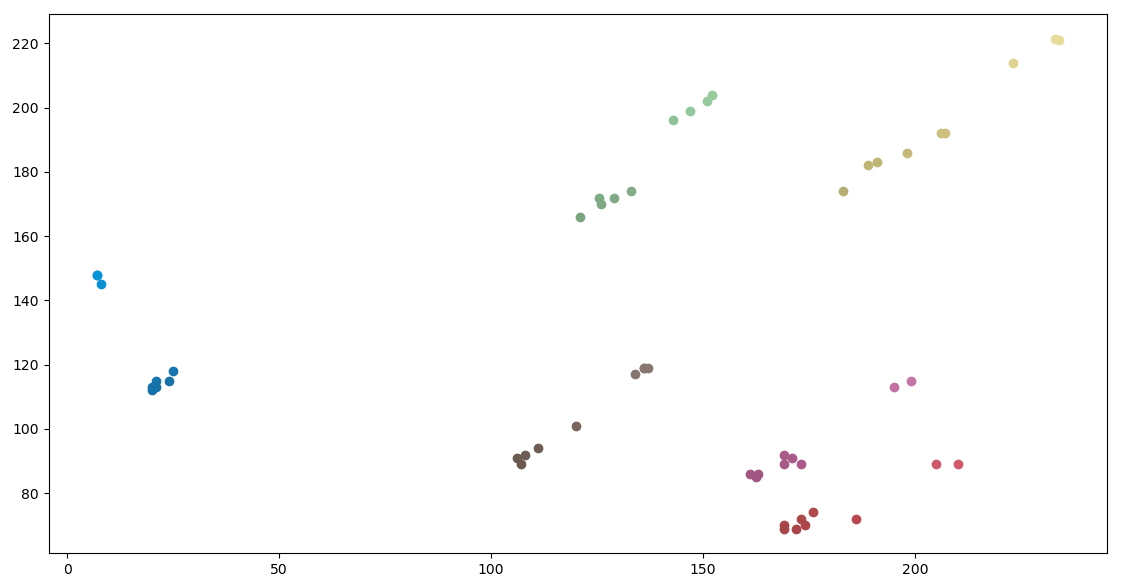
\includegraphics[width=0.80\textwidth]{figures/rg}
	}%
	\vfill
	\subcaptionbox{Proyección en ejes rojo (horizontal) y azul (vertical).}{%
	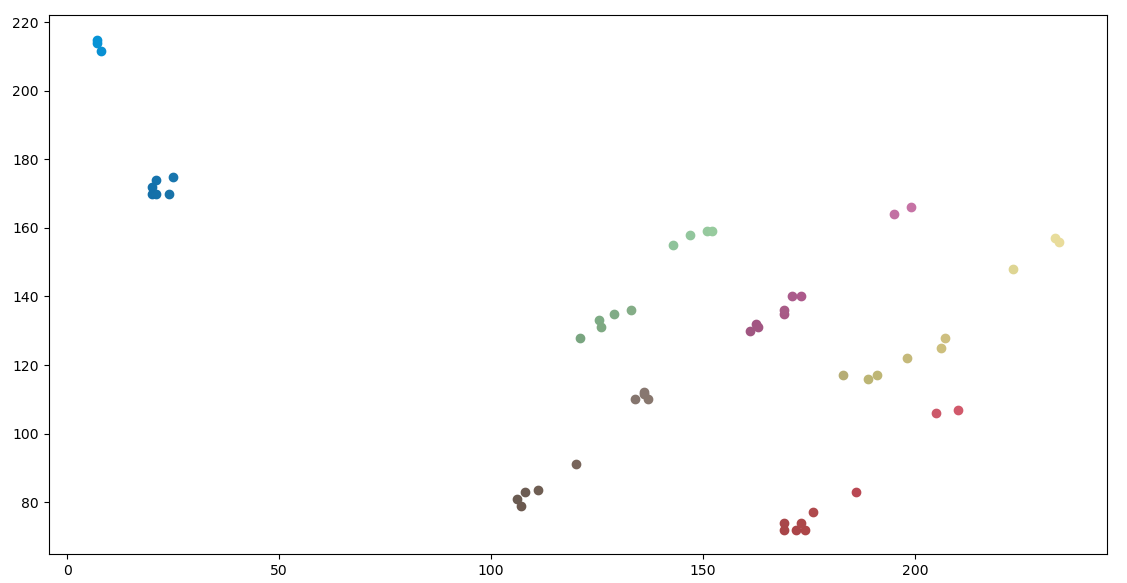
\includegraphics[width=0.80\textwidth]{figures/rb}
	}%
	\vfill
	\subcaptionbox{Proyección en ejes verde (horizontal) y azul (vertical).}{%
	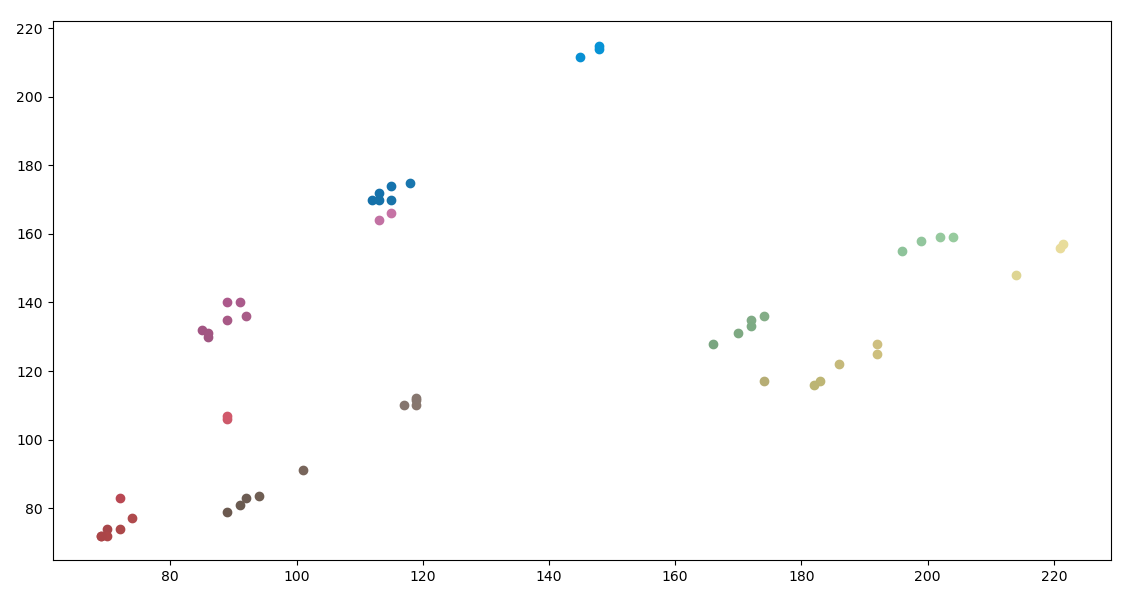
\includegraphics[width=0.80\textwidth]{figures/gb}
	}%
	\caption{Proyecciones .}
	\label{proyecciones}
\end{figure}
